\smallframetitle

\section{Semaine du 03/06/24 au 06/06/24}
\insertsectionframe

\subsection{Comparaison des résultats de 2 détection de villes}
\insertsubsectionframe

\begin{frame}{Affichage}
    \begin{columns}
        \begin{column}{0.5\textwidth}
            \begin{block}{Affichage des différences}
                Afin de visualiser les différences, nous pouvons tracer les 2 classifications en même temps sur une carte en adoptant ce code couleur :
                \begin{itemize}
                    \item Rouge : station en ville dans les 2 classification;
                    \item Bleu : station en ville dans exactement 1 classification;
                    \item Vert : station en campagne dans les 2 classifications.
                \end{itemize}
            \end{block}
        \end{column}

        \begin{column}{0.5\textwidth}
            \begin{figure}
                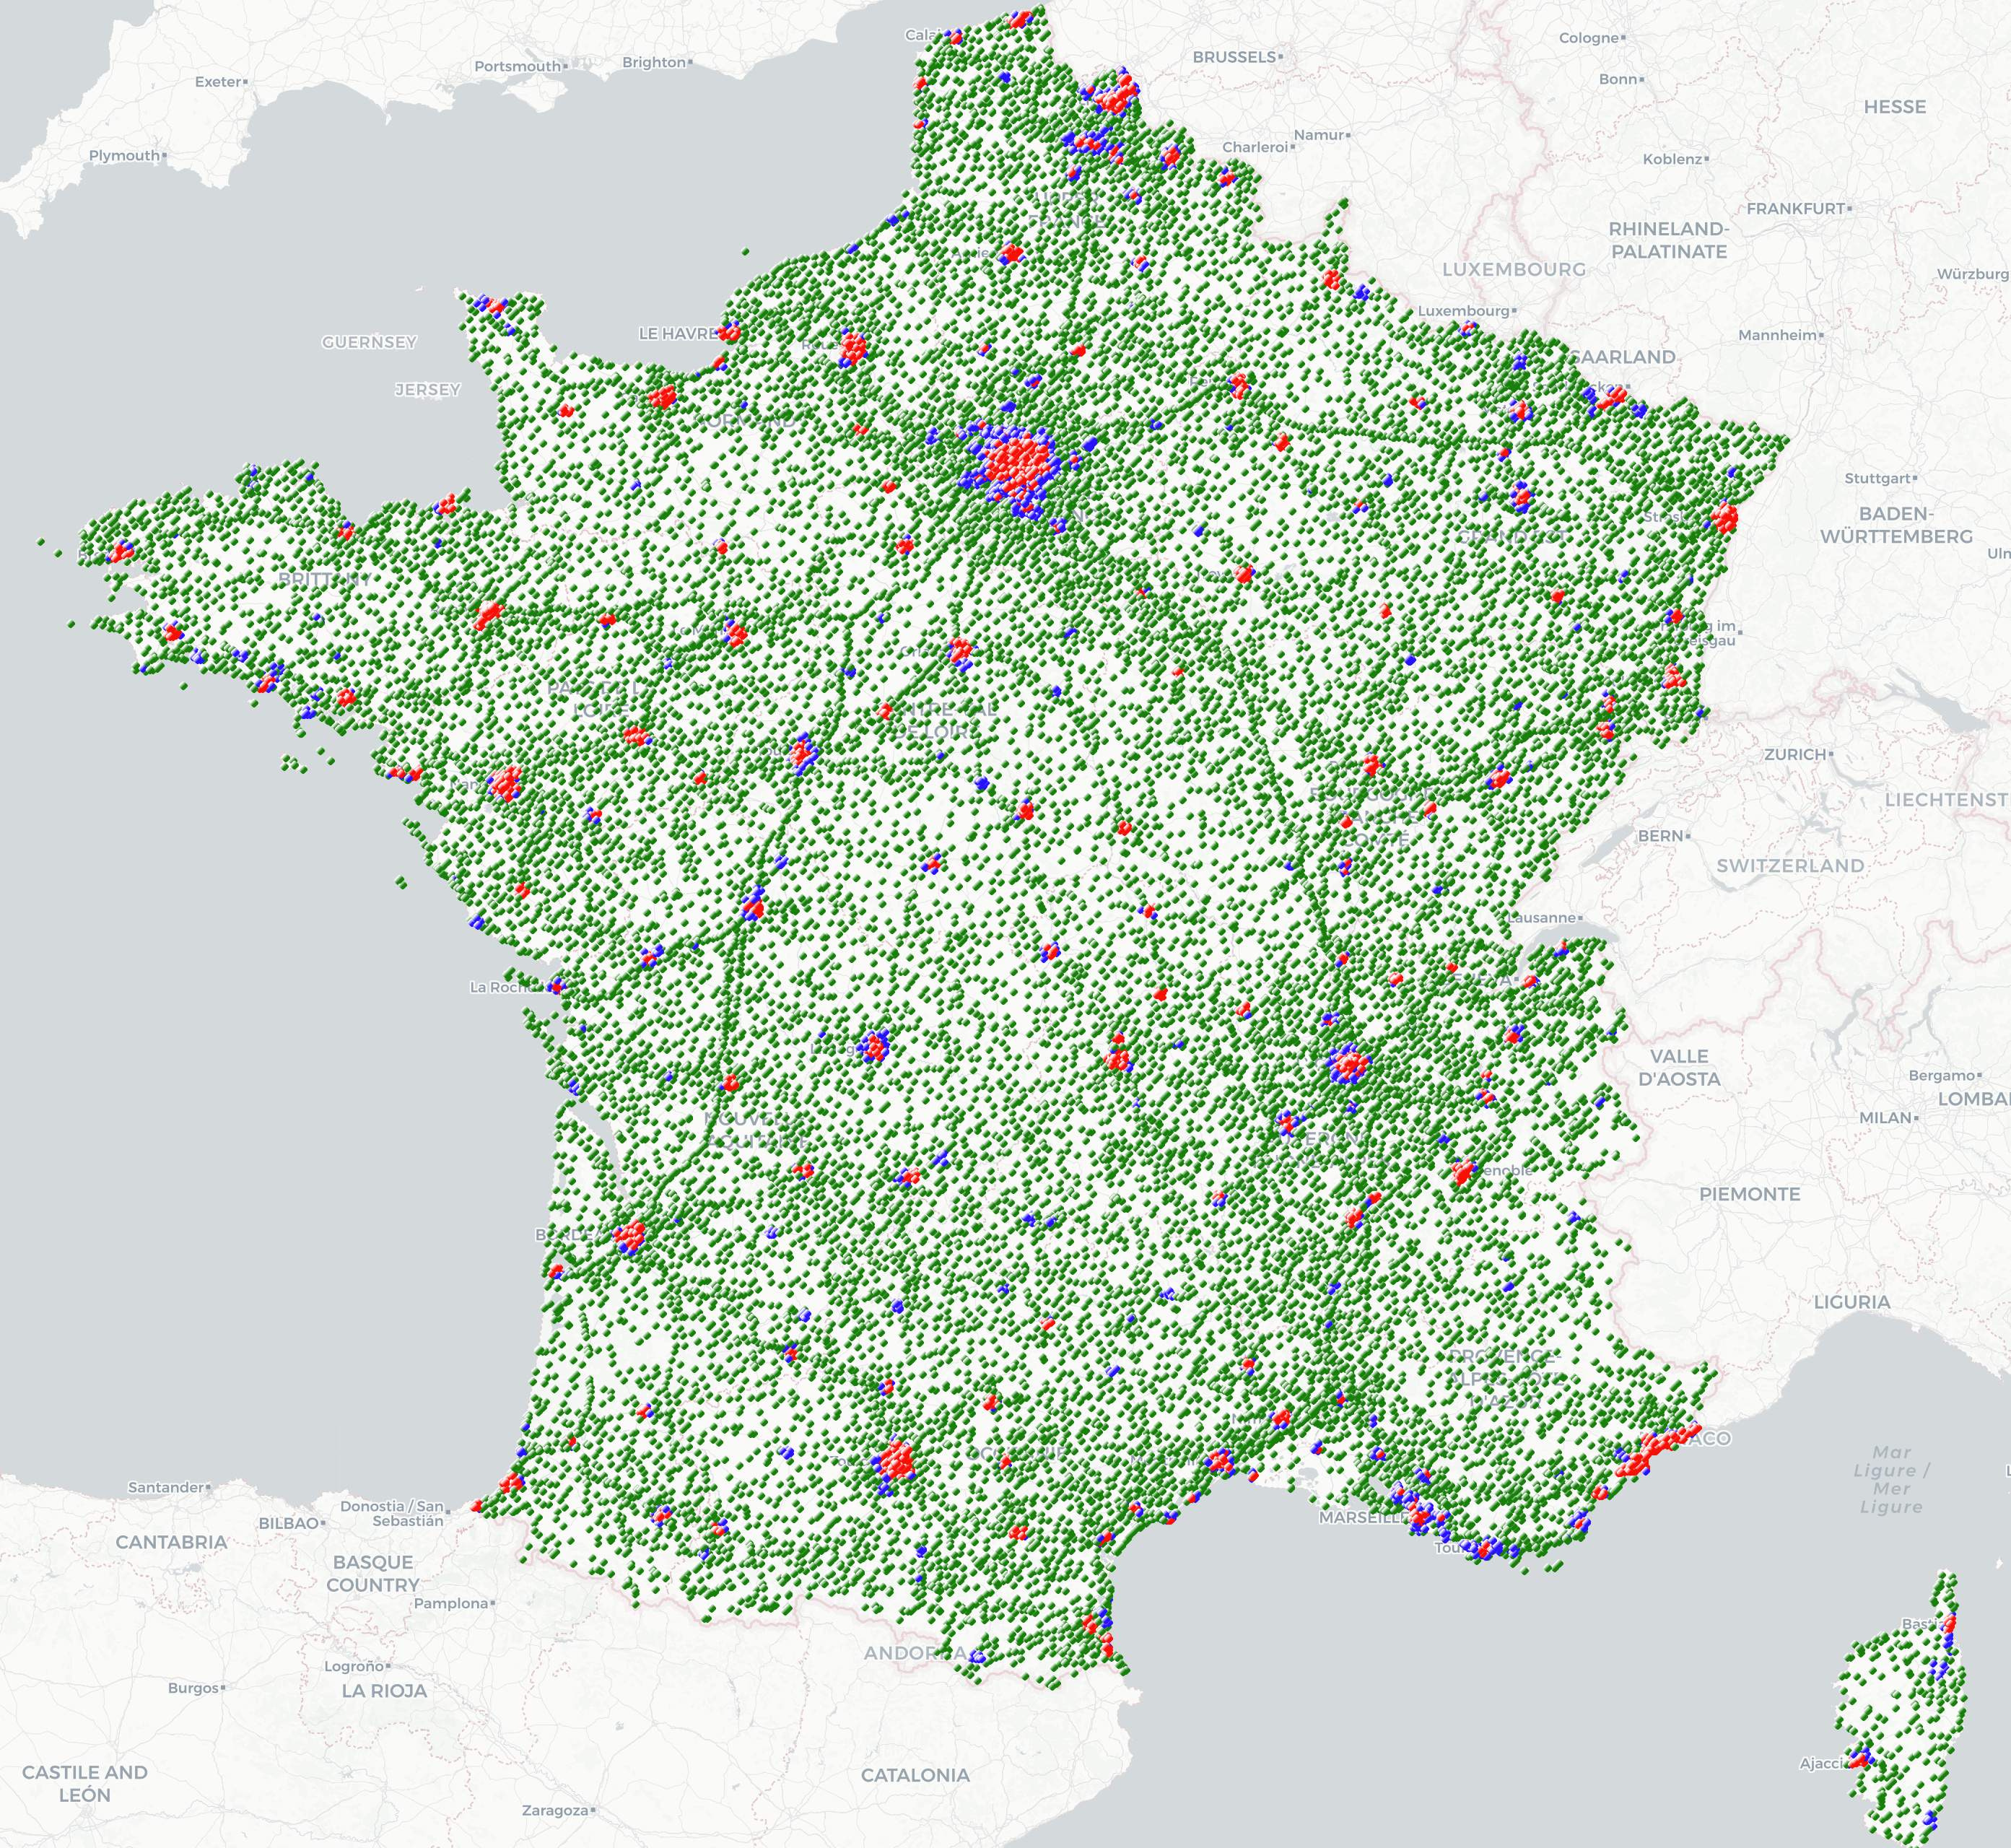
\includegraphics[height=0.5\paperheight]{images/city_comparison.png}
                \caption{\label{fig:city-comparison}Comparaison des résultats de détection de villes : DBScan vs HDBScan}
            \end{figure}
        \end{column}
    \end{columns}
    
    
\end{frame}


\begin{frame}{Indicateurs}
    \begin{block}{Indicateurs de base}
        Nous avons dévéloppé quatre indicateurs de base afin de caractériser la similarité entre deux classifications :
        \begin{itemize}
            \item $a$ : Le pourcentage de station en ville dans les deux classifications;
            \item $b$ : Le pourcentage de station en ville dans la première classifiacation et non la deuxième;
            \item $c$ : Le pourcentage de station en ville dans la deuxième classifiacation et non la première;
            \item $d$ : Le pourcentage de station en campagne dans les deux classifications.
        \end{itemize}
    \end{block}
    \begin{block}{Résultats}
        Sur les classifications présentées dans la slide précédentes, voici les résultats obtenus : 
        \begin{itemize}
            \item $a = 0,688$;
            \item $b = 0,028$;
            \item $c = 0,051$;
            \item $d = 0,232$.
        \end{itemize}
    \end{block}
\end{frame}


\subsection{Nouvelle manière de détecter les villes}
\insertsubsectionframe

\begin{frame}{Changement de cap} 
    \begin{block}{Problèmes rencontrés avec DBScan et HDBScan}
        \begin{itemize}
            \item Méthodes complexes donc peu prévisibles;
            \item Résultats non-satisfaisants quand le méthode est appliquée à seulement une partie de la France.
            \item DBScan est trop binaire, HDBScan est à densité variable donc ne détecte pas toutes les villes de la même façon (problème avec Paris notamment)
            \item Les probabilités de HDBScan ne caractérisent pas exactement la probabilité d'être en ville mais plutôt la certitude avec laquelle on peut rattacher un point à son cluster.
        \end{itemize}
    \end{block}

    \begin{block}{Réflexion sur une méthode plus simple}
        Nous souhaitions savoir quelle station se trouvait en ville, car on sait qu'en ville, les stations sont plus proches les unes des autres, donc les rayons de couverture plus courts.
        Cependant, il n'est pas nécessaire de detecter les villes pour cela, nous pouvons simplement regarder la distance moyenne aux $k$ plus proches voisins.
    \end{block}

\end{frame}

\begin{frame}{Méthodologie}
    \begin{block}{Nouvelle méthode}
        Au lieu d'utiliser une méthode de clustering, nous allons utiliser quelque chose de plus simple.
        On classifie chaque station selon la distance moyenne aux $3$ plus proches voisins. %2 c'est pas assez pour avoir quelquechose de palapable, 4 augmente trop la distance.
        Soit $d$ cette distance, on regroupe les stations de la manière suivante:
        \begin{itemize}
            \item $d\in\left]0, 1\right]$ : centre ville dense;
            \item $d\in\left]1, 2\right]$ : couronne périhurbaine;
            \item $d\in\left]2, 5\right]$ : campagne;
            \item $d\in\left]5, 10\right]$ : campagne profonde;
            \item $d\in\left]10, \infty\right[$ : trou paumé ou valeur aberrante.
        \end{itemize}
    \end{block}
\end{frame}

\begin{frame}{Méthodologie : choix techniques}
    \begin{block}{Calcul des plus proches voisins}
        Nous utilisons la bibliothèque \emph{sklearn.neighbors.NearestNeighbors}\footnotemark.
    \end{block}

    \begin{block}{Choix du nombre de voisins}
        Après plusieurs expérimentations, nous avons choisi de conserver $3$ voisins dans notre calcul.
        En effet, un chiffre inférieur à $2$ serait aberrant car ce ne serait pas une vraie moyenne (ici on cherche plus une mesure de la densité de stations).
        De plus, un chiffre supérieur à $4$ prendrait en compte des stations trop éloignées, ce qui serait aberrant.
    \end{block}
    
    \begin{block}{Métrique}
        Nous avons décidé de partir de la projection de Lambert 93 (qui est déjà présente dans nos données) pour calculer cette distance.
        L'avantage est le gain de temps (environ 30 fois plus rapide), sans perte de performance, par rapport à la conversion en $\unit{km}$ depuis les coordonnées Longitude, Latitude.
    \end{block}

    \footnotetext{\url{https://scikit-learn.org/stable/modules/generated/sklearn.neighbors.NearestNeighbors.html}}
\end{frame}

\begin{frame}{Mise à jour des critères}
    \begin{columns}
        \begin{column}{0.4\paperwidth}
            \begin{block}{Angle}
                Voici les différents paliers que nous appliquons :
                \begin{itemize}
                    \item $d\in\left]0, 1\right]$ : $\text{angle\_min}=40^\circ$;
                    \item $d\in\left]1, 2\right]$ : $\text{angle\_min}=30^\circ$;
                    \item $d\in\left]2, 5\right]$ : $\text{angle\_min}=25^\circ$;
                    \item $d\in\left]5, 10\right]$ : $\text{angle\_min}=15^\circ$;
                    \item $d\in\left]10, \infty\right[$ : $\text{angle\_min}=10^\circ$.
                \end{itemize}
            \end{block}
        \end{column}
        \begin{column}{0.4\paperwidth}
            \begin{block}{Distance}
                Voici les différents paliers que nous appliquons :
                \begin{itemize}
                    \item $d\in\left]0, 1\right]$ : $\text{distance\_max}=\unit[2]{km}$;
                    \item $d\in\left]1, 2\right]$ : $\text{distance\_max}=\unit[5]{km}$;
                    \item $d\in\left]2, 5\right]$ : $\text{distance\_max}=\unit[10]{km}$;
                    \item $d\in\left]5, 10\right]$ : $\text{distance\_max}=\unit[15]{km}$;
                    \item $d\in\left]10, \infty\right[$ : $\text{distance\_max}=\unit[15]{km}$.
                \end{itemize}
            \end{block}
        \end{column}
    \end{columns}
\end{frame}